% !TEX encoding = UTF-8 Unicode
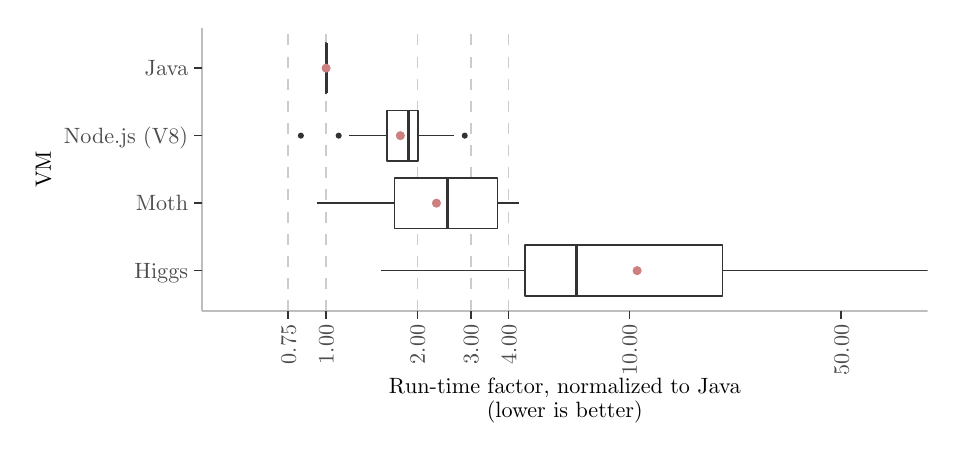
\begin{tikzpicture}[x=1pt,y=1pt]
\definecolor{fillColor}{RGB}{255,255,255}
\path[use as bounding box,fill=fillColor,fill opacity=0.00] (0,0) rectangle (325.21,144.54);
\begin{scope}
\path[clip] ( 62.92, 42.11) rectangle (325.21,144.54);
\definecolor{drawColor}{gray}{0.80}

\path[draw=drawColor,line width= 0.6pt,dash pattern=on 4pt off 4pt ,line join=round] ( 94.14, 42.11) -- ( 94.14,144.54);

\path[draw=drawColor,line width= 0.6pt,dash pattern=on 4pt off 4pt ,line join=round] (107.83, 42.11) -- (107.83,144.54);

\path[draw=drawColor,line width= 0.6pt,dash pattern=on 4pt off 4pt ,line join=round] (140.82, 42.11) -- (140.82,144.54);

\path[draw=drawColor,line width= 0.6pt,dash pattern=on 4pt off 4pt ,line join=round] (160.11, 42.11) -- (160.11,144.54);

\path[draw=drawColor,line width= 0.6pt,dash pattern=on 4pt off 4pt ,line join=round] (173.80, 42.11) -- (173.80,144.54);
\definecolor{drawColor}{gray}{0.20}

\path[draw=drawColor,line width= 0.6pt,line join=round] (251.09, 56.74) -- (325.21, 56.74);

\path[draw=drawColor,line width= 0.6pt,line join=round] (179.71, 56.74) -- (127.70, 56.74);
\definecolor{fillColor}{RGB}{255,255,255}

\path[draw=drawColor,line width= 0.6pt,line join=round,line cap=round,fill=fillColor] (251.09, 47.59) --
	(179.71, 47.59) --
	(179.71, 65.89) --
	(251.09, 65.89) --
	(251.09, 47.59) --
	cycle;

\path[draw=drawColor,line width= 1.1pt,line join=round] (198.42, 47.59) -- (198.42, 65.89);

\path[draw=drawColor,line width= 0.6pt,line join=round] (169.72, 81.13) -- (177.61, 81.13);

\path[draw=drawColor,line width= 0.6pt,line join=round] (132.50, 81.13) -- (104.61, 81.13);

\path[draw=drawColor,line width= 0.6pt,line join=round,line cap=round,fill=fillColor] (169.72, 71.98) --
	(132.50, 71.98) --
	(132.50, 90.27) --
	(169.72, 90.27) --
	(169.72, 71.98) --
	cycle;

\path[draw=drawColor,line width= 1.1pt,line join=round] (151.54, 71.98) -- (151.54, 90.27);
\definecolor{fillColor}{gray}{0.20}

\path[draw=drawColor,line width= 0.4pt,line join=round,line cap=round,fill=fillColor] (157.94,105.52) circle (  0.89);

\path[draw=drawColor,line width= 0.4pt,line join=round,line cap=round,fill=fillColor] (112.38,105.52) circle (  0.89);

\path[draw=drawColor,line width= 0.4pt,line join=round,line cap=round,fill=fillColor] ( 98.72,105.52) circle (  0.89);

\path[draw=drawColor,line width= 0.6pt,line join=round] (141.06,105.52) -- (154.23,105.52);

\path[draw=drawColor,line width= 0.6pt,line join=round] (129.86,105.52) -- (115.96,105.52);
\definecolor{fillColor}{RGB}{255,255,255}

\path[draw=drawColor,line width= 0.6pt,line join=round,line cap=round,fill=fillColor] (141.06, 96.37) --
	(129.86, 96.37) --
	(129.86,114.66) --
	(141.06,114.66) --
	(141.06, 96.37) --
	cycle;

\path[draw=drawColor,line width= 1.1pt,line join=round] (137.61, 96.37) -- (137.61,114.66);
\definecolor{fillColor}{gray}{0.20}

\path[draw=drawColor,line width= 0.4pt,line join=round,line cap=round,fill=fillColor] (107.83,129.91) circle (  0.89);

\path[draw=drawColor,line width= 0.6pt,line join=round] (107.83,129.91) -- (107.83,129.91);

\path[draw=drawColor,line width= 0.6pt,line join=round] (107.83,129.91) -- (107.83,129.91);
\definecolor{fillColor}{RGB}{255,255,255}

\path[draw=drawColor,line width= 0.6pt,line join=round,line cap=round,fill=fillColor] (107.83,120.76) --
	(107.83,120.76) --
	(107.83,139.05) --
	(107.83,139.05) --
	(107.83,120.76) --
	cycle;

\path[draw=drawColor,line width= 1.1pt,line join=round] (107.83,120.76) -- (107.83,139.05);
\definecolor{drawColor}{RGB}{206,128,128}
\definecolor{fillColor}{RGB}{206,128,128}

\path[draw=drawColor,line width= 0.4pt,line join=round,line cap=round,fill=fillColor] (220.22, 56.74) circle (  1.43);

\path[draw=drawColor,line width= 0.4pt,line join=round,line cap=round,fill=fillColor] (147.71, 81.13) circle (  1.43);

\path[draw=drawColor,line width= 0.4pt,line join=round,line cap=round,fill=fillColor] (134.67,105.52) circle (  1.43);

\path[draw=drawColor,line width= 0.4pt,line join=round,line cap=round,fill=fillColor] (107.83,129.91) circle (  1.43);
\end{scope}
\begin{scope}
\path[clip] (  0.00,  0.00) rectangle (325.21,144.54);
\definecolor{drawColor}{RGB}{190,190,190}

\path[draw=drawColor,line width= 0.6pt,line join=round] ( 62.92, 42.11) --
	( 62.92,144.54);
\end{scope}
\begin{scope}
\path[clip] (  0.00,  0.00) rectangle (325.21,144.54);
\definecolor{drawColor}{gray}{0.30}

\node[text=drawColor,anchor=base east,inner sep=0pt, outer sep=0pt, scale=  0.80] at ( 57.97, 53.99) {Higgs};

\node[text=drawColor,anchor=base east,inner sep=0pt, outer sep=0pt, scale=  0.80] at ( 57.97, 78.37) {Moth};

\node[text=drawColor,anchor=base east,inner sep=0pt, outer sep=0pt, scale=  0.80] at ( 57.97,102.76) {Node.js (V8)};

\node[text=drawColor,anchor=base east,inner sep=0pt, outer sep=0pt, scale=  0.80] at ( 57.97,127.15) {Java};
\end{scope}
\begin{scope}
\path[clip] (  0.00,  0.00) rectangle (325.21,144.54);
\definecolor{drawColor}{gray}{0.20}

\path[draw=drawColor,line width= 0.6pt,line join=round] ( 60.17, 56.74) --
	( 62.92, 56.74);

\path[draw=drawColor,line width= 0.6pt,line join=round] ( 60.17, 81.13) --
	( 62.92, 81.13);

\path[draw=drawColor,line width= 0.6pt,line join=round] ( 60.17,105.52) --
	( 62.92,105.52);

\path[draw=drawColor,line width= 0.6pt,line join=round] ( 60.17,129.91) --
	( 62.92,129.91);
\end{scope}
\begin{scope}
\path[clip] (  0.00,  0.00) rectangle (325.21,144.54);
\definecolor{drawColor}{RGB}{190,190,190}

\path[draw=drawColor,line width= 0.6pt,line join=round] ( 62.92, 42.11) --
	(325.21, 42.11);
\end{scope}
\begin{scope}
\path[clip] (  0.00,  0.00) rectangle (325.21,144.54);
\definecolor{drawColor}{gray}{0.20}

\path[draw=drawColor,line width= 0.6pt,line join=round] ( 94.14, 39.36) --
	( 94.14, 42.11);

\path[draw=drawColor,line width= 0.6pt,line join=round] (107.83, 39.36) --
	(107.83, 42.11);

\path[draw=drawColor,line width= 0.6pt,line join=round] (140.82, 39.36) --
	(140.82, 42.11);

\path[draw=drawColor,line width= 0.6pt,line join=round] (160.11, 39.36) --
	(160.11, 42.11);

\path[draw=drawColor,line width= 0.6pt,line join=round] (173.80, 39.36) --
	(173.80, 42.11);

\path[draw=drawColor,line width= 0.6pt,line join=round] (217.41, 39.36) --
	(217.41, 42.11);

\path[draw=drawColor,line width= 0.6pt,line join=round] (294.00, 39.36) --
	(294.00, 42.11);
\end{scope}
\begin{scope}
\path[clip] (  0.00,  0.00) rectangle (325.21,144.54);
\definecolor{drawColor}{gray}{0.30}

\node[text=drawColor,rotate= 90.00,anchor=base east,inner sep=0pt, outer sep=0pt, scale=  0.80] at ( 96.89, 37.16) {0.75};

\node[text=drawColor,rotate= 90.00,anchor=base east,inner sep=0pt, outer sep=0pt, scale=  0.80] at (110.58, 37.16) {1.00};

\node[text=drawColor,rotate= 90.00,anchor=base east,inner sep=0pt, outer sep=0pt, scale=  0.80] at (143.57, 37.16) {2.00};

\node[text=drawColor,rotate= 90.00,anchor=base east,inner sep=0pt, outer sep=0pt, scale=  0.80] at (162.87, 37.16) {3.00};

\node[text=drawColor,rotate= 90.00,anchor=base east,inner sep=0pt, outer sep=0pt, scale=  0.80] at (176.56, 37.16) {4.00};

\node[text=drawColor,rotate= 90.00,anchor=base east,inner sep=0pt, outer sep=0pt, scale=  0.80] at (220.16, 37.16) {10.00};

\node[text=drawColor,rotate= 90.00,anchor=base east,inner sep=0pt, outer sep=0pt, scale=  0.80] at (296.75, 37.16) {50.00};
\end{scope}
\begin{scope}
\path[clip] (  0.00,  0.00) rectangle (325.21,144.54);
\definecolor{drawColor}{RGB}{0,0,0}

\node[text=drawColor,anchor=base,inner sep=0pt, outer sep=0pt, scale=  0.80] at (194.07, 12.46) {Run-time factor, normalized to Java};

\node[text=drawColor,anchor=base,inner sep=0pt, outer sep=0pt, scale=  0.80] at (194.07,  3.82) {(lower is better)};
\end{scope}
\begin{scope}
\path[clip] (  0.00,  0.00) rectangle (325.21,144.54);
\definecolor{drawColor}{RGB}{0,0,0}

\node[text=drawColor,rotate= 90.00,anchor=base,inner sep=0pt, outer sep=0pt, scale=  0.80] at (  8.36, 93.32) {VM};
\end{scope}
\end{tikzpicture}
